\chapterstart{第三阶段：原理指导的模型改进}
\label{sec:guided}

第三阶段回到第一代模型。此时已有两项重要认识：文本出现于输入，不保证模型会使用其中的关系；学会一种新行为，也不保证原有功能仍然完好。Qiushi Engine 因此沿用 \Frontier{} 的权重、分词器、残差结构和既有文本，重点改变训练任务本身：让哪些提示可见，要求预测哪些词，以及怎样限制对原有预测的破坏。最后再与普通续训比较，判断这些设计是否真正改善模型。

\subsection{从机制判断到可执行设计}

第二阶段的关系实验表明，来源是否进入预测窗口会改变模型学习到的来源利用行为；监督与功能干预又表明，可见信息不一定被有效使用，熟悉表现也不能代替调用能力的检验。由这些认识出发，真实训练中的设计问题被收束为三个变量（表\ref{tab:bridge}）。

\begin{table}[htbp]
\caption{科学认识与训练设计的对应。每项认识落实为具体训练改动，并由相应对照和行为测量检验。}
\label{tab:bridge}
\small
\begin{tabularx}{\linewidth}{@{}Y Y Y@{}}
\toprule 研究认识 & 训练改动 & 直接检验\\\midrule
来源可见不保证被使用 & 保留来源，削弱重述侧的局部线索 & 固定目标、改变遮盖；测量来源条件差异\\
监督数量与输入条件是不同变量 & 密集遮盖，但仅监督选定的稀疏目标 & 比较稀疏与密集目标；完成真实模型评测\\
保持约束可能同时限制新学习 & 在普通输入上保持母模型功能 & 比较密集输入与普通输入的新学习、预测变化及任务结果\\
\bottomrule
\end{tabularx}
\end{table}

方案的形成经历了具体的判断更新。早期研究将收益较多地归于增加预测目标；固定稀疏目标后，扩大输入遮盖仍观察到效果，因而转向分别研究可见信息与监督数量。普通输入保持方案形成后，研究再比较不同保持输入与更新幅度，检验它们怎样影响新学习。这是一项逐轮提出判断、设计对照并修正解释的研究，而非在全部实验之前一次性确定整套方案。

\subsection{分别设计可见输入与监督目标}

来源—重述配对沿用第一阶段已有数据，不在本轮重新生成改写。普通整词遮盖只隐藏部分词，重述内部可能仍保留足够提示，使模型不读来源也能预测目标。新方案保留来源，隐藏重述中的更多候选词，但只选择其中一部分计算预测错误、用于更新参数。候选词按字符位置对应到一个或多个 token，这些一起处理的单元称为内容组。

遮盖与监督分别控制两件事：前者改变模型能看见什么，后者决定哪些位置的预测错误参与训练。一个位置可以被遮盖而不计入预测损失，用来去除其他目标附近的线索。本文的密集遮盖、稀疏监督正是这一安排：扩大线索缺失范围，同时保留较小的预测目标集合。

以 $(I,T)$ 表示输入遮盖与监督目标的组合，$S$ 表示稀疏，$M$ 表示密集。本文将专门选定用于来源—重述预测的位置称为聚焦目标，对这些位置计算的预测损失称为聚焦损失。$(S,S)$ 与 $(M,S)$ 使用同样的稀疏聚焦目标，区分局部可见线索；$(M,S)$ 与 $(M,M)$ 使用密集遮盖输入，区分哪些遮盖位置承担聚焦损失。图\ref{fig:mask}说明这一差别。

\begin{figure}[htbp]
\centering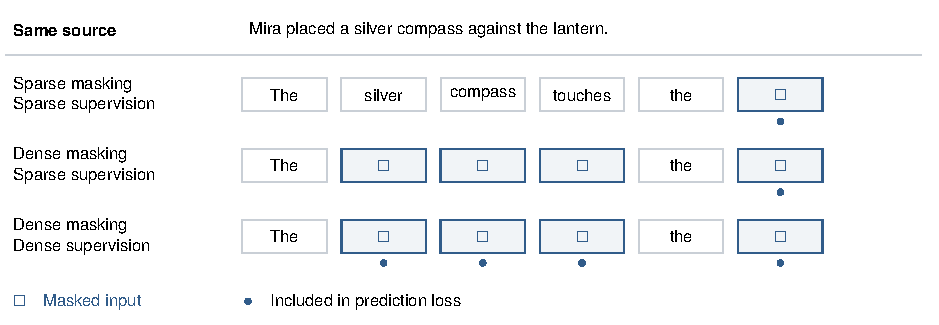
\includegraphics[width=\linewidth]{figures/input_supervision.pdf}
\caption{输入遮盖与监督目标的分离：词级示意。基于同一示例来源—重述对，前两行固定监督目标、改变遮盖范围，后两行固定遮盖范围、改变监督目标。空方框表示被遮盖词，圆点表示计入预测损失的位置。候选内容词参与选择，停用词保持可见；实际选词与分词规则见附录\ref{app:repro}。}
\label{fig:mask}
\end{figure}

本轮训练文本包含 20,475 行、3,162,742 词。一行是装填成训练输入的文本，可以包含多个片段；用于聚焦关系预测的 3,831 行既有 Qwen 改写，包含 11,778 个配对片段。这些行采用密集遮盖、稀疏监督，其余行继续承担普通语言预测，包括第一阶段的紧凑重述与预算再分配材料。密集遮盖涉及 132,283 个内容组、176,607 个 token；稀疏监督选择 21,479 个内容组、28,590 个 token。因此，$(M,S)$ 中有 148,017 个 token 虽被遮盖，却不计入这部分预测损失。稀疏与密集相对于候选集合定义，确切选择规则见附录\ref{app:repro}。

新学习目标将关系预测与普通语言预测结合：
\begin{equation}
 \mathcal L_{\mathrm{acq}}
 =0.15\,\overline{\CE}_{\mathrm{focus}}
 +0.85\,\overline{\CE}_{\mathrm{ordinary}}.
\label{eq:acquisition}
\end{equation}
其中 $\overline{\CE}_{\mathrm{focus}}$ 是选定关系目标上的平均预测损失，$\overline{\CE}_{\mathrm{ordinary}}$ 是普通目标上的平均预测损失。每次参数更新先汇集相应训练行，再各自按全部有效目标 token 取均值，按 0.15 与 0.85 加权；不是先对每行或每个微批次等权平均。这些系数表示两类学习信号的权重，而非文本比例。普通目标使模型在练习关系预测时，仍继续学习更广泛的语言规律。

输入遮盖与预测监督的分离已有直接研究\citep{wettig2023mask}。本研究将这一设计用于来源—重述关系：来源保持可见，通过遮盖重述侧的局部线索改变预测条件，同时单独选择承担损失的目标。相应对照用于辨明这些操作改变了什么行为，以及能否在第一代模型上产生实际收益。

\subsection{在普通输入条件下保持功能}

新的训练任务允许模型在大量局部线索缺失时改变预测方式，同时需要保存普通语言输入上的已有功能。保持方案将用于关系学习的既有 Qwen 配对行再次呈现，但改用普通 15\% 整词遮盖；更新后的模型与冻结的 \Frontier{} 对同样输入和目标位置作预测。两者的概率分布差异用 KL 散度衡量：差异越小，保持损失越低。第一代模型的输出由此成为继续学习中的功能参照。“普通输入”描述这里的遮盖方式，并非另引入一套语料。

具体目标为
\begin{align}
 \mathcal L_{\mathrm{pres}}
 &=\frac{1}{|Q_p|}\sum_{(x,i)\in Q_p}
   \KL\!\left(p_{\Frontier}(\cdot\mid x,i)\,\|\,p_\theta(\cdot\mid x,i)\right),\\
 \mathcal L&=\mathcal L_{\mathrm{acq}}+\lambda\mathcal L_{\mathrm{pres}},
 \qquad\lambda=1,\quad T=1.
\label{eq:preservation}
\end{align}
式中 $x$ 是施加普通整词遮盖后的完整行，$i$ 是该行被选为普通预测目标的位置，$Q_p$ 汇集本次更新中全部保持目标。KL 在这些位置的整个词表概率分布上计算，再按目标总数平均，不约束所有可见位置。$p_{\Frontier}$ 是冻结第一代模型的预测分布，$p_\theta$ 是待更新模型的预测分布，$\lambda$ 控制保持约束的权重。温度 $T$ 控制分布计算前的得分缩放，取 1 时不额外缩放。提供参照的模型称为教师，被更新的模型称为学生；这里的教师就是第一代模型。

比较输出时需要排除运行随机性。神经网络训练中的 dropout 会随机屏蔽部分计算，若两个模型使用不同随机状态，即使权重相同，输出也可能不同。因此，保持分支采用确定性计算，并保存、恢复随机数状态，避免额外计算扰动原训练。这使“输出发生变化”主要反映模型更新，而不是比较程序本身带来的随机差别。

以旧模型输出约束后续学习，与 Learning without Forgetting 等方法直接相关\citep{li2016learning}。第一代已经采用 KL 保持项，本阶段进一步研究保持的作用条件：让模型在新的预测任务中学会改变，同时减少普通输入上不必要的功能变化。

第三阶段仍只更新既有增量分支的 995,584 个参数，固定残差尺度为 0.75，不改变总参数量。完整方案采用 80 次参数更新，除新学习曝光外增加 517,332 词普通输入呈现：
\begin{equation}
 86{,}005{,}295+3{,}162{,}742+517{,}332=89{,}685{,}369.
\label{eq:budget}
\end{equation}
无保持分支的对照累计为 89,168,037 词。完整方案额外呈现的 517,332 词，相当于本轮新学习词数的 16.36\%，并增加了前向计算。两类方案均在 100M 词上限内；下文将不增加保持呈现的训练设计收益与包含额外保持训练的整体收益分别报告。

\subsection{完整评测与续训重复}
\label{sec:complete_results}

表\ref{tab:strategies}汇总共同母模型和四种训练策略的完整九项评测。每种策略采用续训种子 62064 和 62065，两次训练共享同一预训练起点，改变后续训练的随机过程。普通续训作为实践参照，检验新设计是否产生超过继续训练本身的收益。固定稀疏目标的 $(S,S)$ 则用于输入条件的机制比较，两类对照承担不同任务。

\begin{table}[htbp]
\caption{共同母模型与四种续训策略的完整 Overall。两列为同一预训练起点上的续训重复。完整策略包含额外的保持性文本呈现，全部九项分数见附录\ref{app:local}。}
\label{tab:strategies}
\small
\begin{tabularx}{\linewidth}{@{}Yrrr@{}}
\toprule 训练策略 & 种子 62064 & 种子 62065 & 累计词曝光\\\midrule
\input{tables/strategies}
\end{tabularx}
\end{table}

\begin{figure}[htbp]
\centering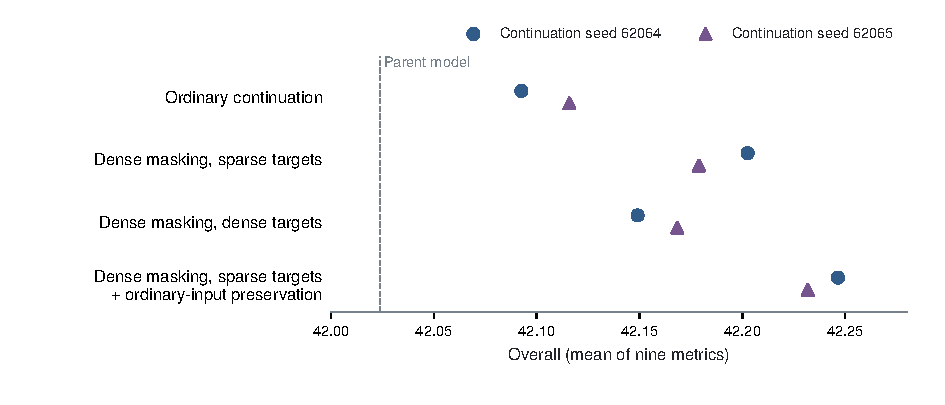
\includegraphics[width=\linewidth]{figures/strategy_comparison.pdf}
\caption{同一母模型上不同续训策略的完整评测。圆点与三角分别表示续训种子 62064 和 62065，虚线表示母模型的 Overall。各候选均完成九项评测；完整保持策略包含额外的普通输入呈现（表\ref{tab:strategies}）。}
\label{fig:strategies}
\end{figure}

$(M,S)$ 相对普通续训分别提高 0.1099 与 0.0630，在相同累计词曝光下得到一致方向的完整评测收益。完整策略相对普通续训分别提高 0.1538 与 0.1158，相对 $(M,S)$ 再提高 0.0439 与 0.0529。两个密集监督 $(M,M)$ 模型低于同种子的稀疏监督 $(M,S)$：在聚焦损失总权重固定为 0.15 时，把监督分配到更多目标，并未带来更好的综合结果。这一区别涉及目标集合及单个目标获得的相对权重。

这些比较给出两个层次的结果：相同累计曝光下，$(M,S)$ 优于普通续训；加入普通输入保持后，完整方案进一步改善。$(S,S)$ 现有结果为快速评测和机制测量，未列入完整九项表，因此局部遮盖作用的归因应依据相应机制对照，不能由 $(M,S)$ 与普通续训的 Overall 差值单独确定。

图\ref{fig:contributions}进一步分解完整策略相对母模型的变化。各分项变化除以 9，即为其对 Overall 的贡献。GlobalPIQA 是最大的增益来源，对两个模型的贡献均约为 0.165，占总增量的约 74\% 与 79\%。实体跟踪等分项也有提高，另一些分项下降；其余八项合计对 Overall 贡献 0.0574 与 0.0428。分项分解说明，新方法的净收益来自具体能力的改善及其间的取舍。

若问新设计比普通续训改善了什么，则需以普通续训为参照。此时，实体跟踪对 Overall 的贡献分别为 $+0.1378$ 和 $+0.1511$，是两个种子最大的正向变化；GlobalPIQA 均贡献 $+0.0572$，其他分项合计则抵消部分收益。进一步比较完整策略与不加保持的 $(M,S)$，GlobalPIQA 分数完全相同，额外的 $+0.0439$ 与 $+0.0529$ 来自其他分项的净改善。因此，相对母模型的能力增量、相对普通续训的方法收益，以及保持方案带来的附加变化，应分别解释。

对下游微调的补充复核也已有结果：在微调种子 42 和 44 下，完整方案的 (Super)GLUE 均值都高于母模型和 $(M,S)$。这项比较固定续训模型、改变下游微调的随机过程，与前述两个续训种子检验不同来源的随机性；三种模型的对应结果见表\ref{tab:finetuning_seeds}。

\begin{figure}[htbp]
\centering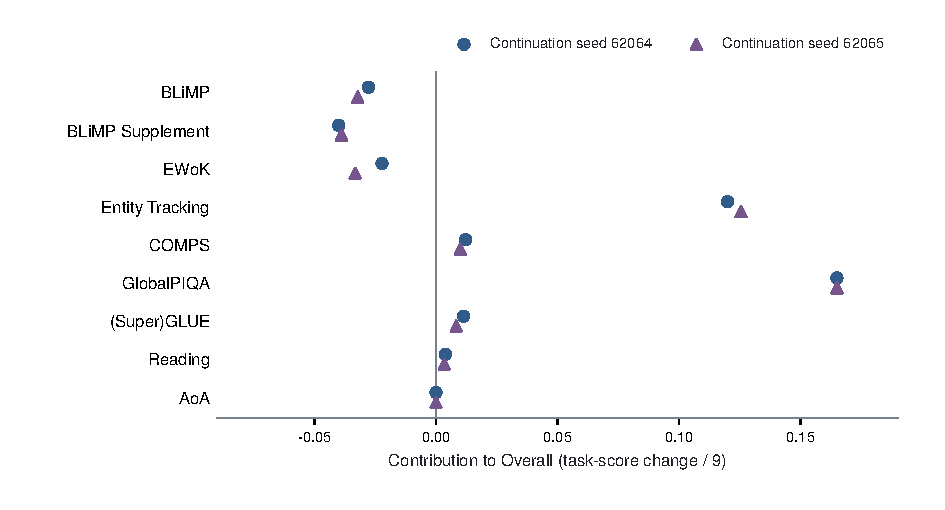
\includegraphics[width=\linewidth]{figures/task_contributions.pdf}
\caption{完整策略的分项收益与代价。以共同母模型为参照，各分项分数变化除以 9，得到其对 Overall 变化的贡献。圆点与三角分别对应续训种子 62064 和 62065，图中显示点估计。两个种子使用相同评测集合，其中 GlobalPIQA 包含 203 题。}
\label{fig:contributions}
\end{figure}

\subsection{新能力获得与功能保持的机制分析}

为解释保持如何影响新学习，研究在密集遮盖输入上测量三个量：正确目标的交叉熵、该目标在全部候选词中的排名，以及更新模型与母模型的 KL。较低的交叉熵和更靠前的正确词排名表示预测改善；较小的 KL 表示输出变化较少。比较使用已经训练过的 169 个样本，在共同的 1,003 个目标 token 上进行，因此测量的是已训练行为，而非陌生文档上的泛化。

\begin{table}[htbp]
\caption{密集遮盖输入上的新学习与预测变化。除注明 62065 的一行外，续训种子均为 62064。前两个数值列为相对母模型的改善，越大越好；KL 衡量模型输出变化。最后一行将保持约束施加于密集遮盖输入。}
\label{tab:preservation}
\small
\begin{tabularx}{\linewidth}{@{}Yrrr@{}}
\toprule 方案 & CE 改善（nats） & 排名改善 & 母模型 KL（nats）\\\midrule
普通续训 & $-0.005$ & 0.7 & 0.001\\
不加保持 $(M,S)$ & 0.757 & 132.8 & 0.503\\
完整策略，62064 & 0.682 & 128.3 & 0.353\\
完整策略，62065 & 0.679 & 128.0 & 0.345\\
密集遮盖输入保持 & 0.159 & 34.8 & 0.009\\
\bottomrule
\end{tabularx}
\end{table}

普通输入保持保留了大部分新学到的预测改善；在密集遮盖输入上保持，则显著减小了模型变化，也削弱了对正确词的学习收益。这使保持设计的目标更加清楚：限制普通功能的损伤，同时允许新任务所需的预测改变。研究随后进一步检查，不同输入上的约束实际有多强。

这项比较固定同一更新模型和母模型，在上述共同位置上测量两种输入的差异。密集遮盖使母模型更难预测：表示预测不确定性的熵增加 1.6330 nats，正确目标交叉熵增加 1.3155 nats，两模型间的 KL 增加 0.4738 nats。保持损失对可训练参数产生的梯度大小达到普通输入的 11.835 倍。梯度表示损失要求参数朝什么方向、以多大幅度改变；两个保持梯度的方向相似度为 0.7288，却具有很不同的大小。这解释了为什么使用相同系数不代表施加了同等强度的约束。

\begin{table}[htbp]
\caption{固定模型、共同目标位置上的保持约束比较。更新模型为续训种子 62064 的 $(M,S)$，参照为第一代母模型。前三项为密集遮盖输入减普通遮盖输入的差值，最后一项为保持梯度大小之比。}
\label{tab:gradient_geometry}
\begin{tabularx}{\linewidth}{@{}Yr@{}}
\toprule 共同位置上的比较 & 结果\\\midrule
母模型预测熵差（nats） & $+1.6330$\\
母模型目标交叉熵差（nats） & $+1.3155$\\
教师到学生 KL 差（nats） & $+0.4738$\\
保持梯度范数之比：密集／普通 & $11.835$\\
\bottomrule
\end{tabularx}
\end{table}

完整保持比较还涉及目标位置的变化：普通遮盖条件有 4,762 个目标，密集遮盖输入上未承担聚焦监督的位置有 6,665 个目标，共同部分为上述 1,003 个位置。结果支持保持配置会改变新学习与旧功能的平衡；输入类型、目标集合和有效约束强度的独立作用尚未完全分离。由此得到更具体的设计要求：保持方案应同时说明约束对象、实际强度，以及新能力和原有功能各自的变化。

普通输入上的另一组测量使用 384 个完整既有文本行、10,348 个目标，保留来源并施加普通整词遮盖。不加保持与完整策略的母模型 KL 分别为 0.02449 和 0.00941 nats；相对母模型的 CE 恶化由 0.0290 降至 0.0100 nats。这组结果显示，普通输入保持确实减小了相应功能变化。该组与表\ref{tab:preservation}分别测量普通输入和密集遮盖输入，使用不同样本，各自按共同参照比较。

来源条件干预使用本轮续训文本之后的 96 个来源对、186 个共同目标。这些样本位于本轮训练范围之外，与母模型预训练文档的独立性尚未确认。正确来源下的 NLL 小幅改善，错源、去源条件则出现更明显的预测代价（表\ref{tab:source_final}）。完整策略缓解了部分代价，并保留正确来源下的改善。这项测量刻画模型如何响应来源变化，与关系推理的泛化能力分别评价。

\begin{table}[htbp]
\caption{续训种子 62064 的两个模型在不同来源条件下的预测变化。数值为相对母模型的目标 NLL 差值，单位为 nats，负值表示改善；各条件使用同一组目标。}
\label{tab:source_final}
\begin{tabularx}{\linewidth}{@{}Yrr@{}}
\toprule 来源条件 & 不加保持 $(M,S)$ & 完整策略\\\midrule
正确来源 & $-0.024$ & $-0.022$\\
错误来源 & $+0.149$ & $+0.099$\\
仅保留重述 & $+0.107$ & $+0.076$\\
完整行中擦除当前来源 & $+0.210$ & $+0.127$\\
完整行中擦除全部来源 & $+0.0248$ & $+0.0101$\\
\bottomrule
\end{tabularx}
\end{table}

\subsection{实践检验如何修正原则}

第三阶段验证了认识指导训练的实际作用，也使原则更精确。扩大遮盖范围与增加监督目标产生不同效果，支持分别设计预测条件和学习任务。保持约束需要同时检查新学习与普通功能，不能单以输出接近旧模型作为成功标准。来源干预则进一步说明，新模型怎样利用真实来源，以及在错误来源下付出什么代价。

至此，三阶段形成了连续的方法发展：第一代提供成熟模型与关系文本，第二阶段辨明信息利用和能力复用的条件，第三阶段据此改变输入、监督与保持方式，并取得重复的完整评测改善。实际训练结果使科学认识转化为可采用的方法。

新的实践也改变了后续研究应采用的判断依据。固定目标后的遮盖对照，使输入条件与监督数量得到区分；共同位置上的梯度比较，则说明保持系数相同仍可能对应不同的实际约束。Qiushi Engine 因而不仅保留有效方案，也修正方案的解释，留下更明确的比较条件供后续研究使用。模型改进、方法积累与知识修正在这里相互联系，构成第\ref{sec:rsi}节讨论 Research RSI 的具体依据。
